\section{Entry criteria}
Before proceeding with the integration test in this section we analysed the prerequisites that the software must satisfy.
\\First of all we must have a code-complete project, all modules must be available and their performances and memory requirements have to fit the specifications.
\\Secondly all the modules must be unit tested. 
\\Finally the RASD and DD must be completed, they provide all the documentation that we need for proceeding in the succeeding steps.

\section{Elements to be integrated}
In the Design Document, we identified four main Tiers: the EIS Tier, the Business Tier, the Web Tier and the Client Tier. These are the subsystems that we are going to integrate.
Additionally, the Client tier is composed by the Web Application, the Mobile Application and the On-Board Application. Two main external systems, PaymentHandler and NotificationHandler, are to be integrated with the Business Tier.
\\The subsystems that are to be integrated and their components are exhaustively described in section \ref{sec:integration_sequence} of this document.

\section{Integration testing strategy}
We choose for our integration testing strategy to adopt a bottom-up approach. In this way, we test the subsystems from the lower level to the top level, where all the modules are integrated. 
\\There are different advantages following this strategy. The test conditions for each module are easier to create and the test results can be analysed in a simpler way. Then it's easier to localize problems and faults. In the end we can proceed with the test phase of our subsystems alongside their implementation.
\\On the other side the bottom-up approach brings some disadvantages. The main one is the need of driver programs in order to simulate the missing modules while they aren't already deployed. Another disadvantage is the fact that we can't test the whole program until the last module has been developed. Anyway, we think that these disadvantages are bearable comparing the advantages that this approach provides, a last evidence is the fact that probably almost all the faults occurs toward the bottom of the system.
\\In the testing phase we also selected the order of the subsystems to analyse, not randomly but privileging the critical ones.
\\ We also follow a specific path before performing the integration test. First of all, we design the integration test and the specific drivers if they aren't already done. If it was not made at the unit test we design the input test data, thirdly we set the modules involved, the drivers and the input test data. Finally, we proceed performing the integration test.

\newpage
\section{Sequence of Component/Function Integration} \label{sec:integration_sequence}

	\subsection{Software Integration Sequence}{}
	The following figures (fig.\ref{fig:database_integration}, fig.\ref{fig:application_logic_subsystem}) show the components of the PowerEnJoy system integrated into subsystems, the arrows indicate the order of integration. Every figure is followed by a table which summarizes the related integration tests.

	\begin{figure}[!ht]
	  \centering
	  \vspace{0.2cm}
	  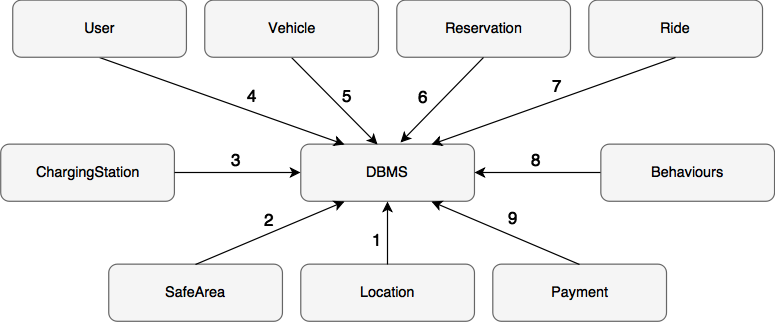
\includegraphics[width=1.0\textwidth]{/ITPD/database_subsystem}\\
	  \vspace{0.2cm}
	  \caption{Integration sequence for the Enterprise-Information-System subsystem} 
	  \label{fig:database_integration} 
	\end{figure}

	\begin{center}
		\vspace{0.6cm}
		\begin{tabular}{|l|l|l|}
			\hline
			\textbf{ID} & \textbf{Integration Test} & \textbf{Paragraphs} \bigstrut \\\hline
			\hline
			I01T1 & Location \ensuremath{\rightarrow} DBMS & \ref{I01}, \ref{TP1} \bigstrut \\\hline
			I01T2 & SafeArea \ensuremath{\rightarrow} DBMS & \ref{I01}, \ref{TP1} \bigstrut \\\hline
			I01T3 & ChargingStation \ensuremath{\rightarrow} DBMS & \ref{I01}, \ref{TP1} \bigstrut \\\hline
			I01T4 & User \ensuremath{\rightarrow} DBMS & \ref{I01}, \ref{TP1} \bigstrut \\\hline
			I01T5 & Vehicle \ensuremath{\rightarrow} DBMS & \ref{I01}, \ref{TP1} \bigstrut \\\hline
			I01T6 & Reservation \ensuremath{\rightarrow} DBMS & \ref{I01}, \ref{TP1} \bigstrut \\\hline
			I01T7 & Ride \ensuremath{\rightarrow} DBMS & \ref{I01}, \ref{TP1} \bigstrut \\\hline
			I01T8 & Behaviours \ensuremath{\rightarrow} DBMS & \ref{I01}, \ref{TP1} \bigstrut \\\hline
			I01T9 & Payment \ensuremath{\rightarrow} DBMS & \ref{I01}, \ref{TP1} \bigstrut \\\hline
		\end{tabular}
	\end{center}

	\newpage
	\begin{figure}[!ht]
	  \centering
	  \vspace{0.2cm}
	  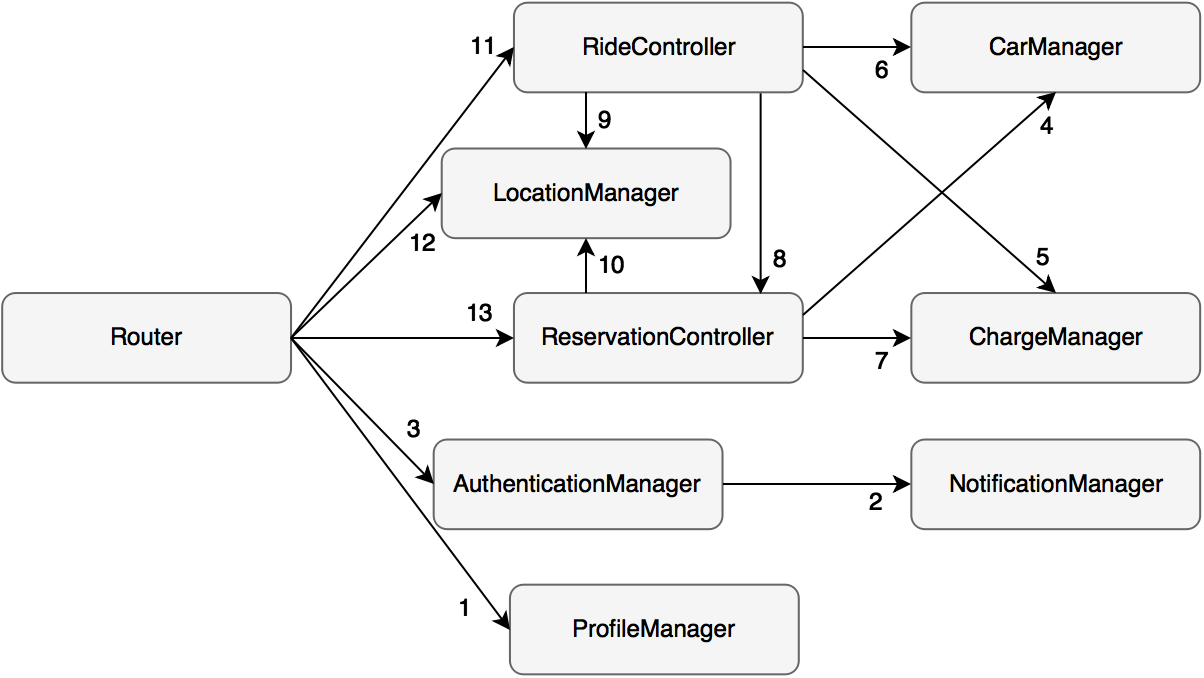
\includegraphics[width=1.0\textwidth]{/ITPD/application_logic_subsystem}\\
	  \vspace{0.2cm}
	  \caption{Integration sequence for the Business subsystem} 
	  \label{fig:application_logic_subsystem} 
	\end{figure}

	\begin{center}
		\vspace{0.6cm}
		\begin{tabular}{|l|l|l|}
			\hline
			\textbf{ID} & \textbf{Integration Test} & \textbf{Paragraphs} \bigstrut \\\hline
			\hline
			I02T1 & Router \ensuremath{\rightarrow} ProfileManager & \ref{I02}, \ref{TP2} \bigstrut \\\hline
			I03T1 & AuthenticationManager \ensuremath{\rightarrow} NotificationManager & \ref{I03}, \ref{TP2} \bigstrut \\\hline
			I04T1 & Router \ensuremath{\rightarrow} AuthenticationManager & \ref{I04}, \ref{TP2} \bigstrut \\\hline
			I05T1 & ReservationController \ensuremath{\rightarrow} CarManager & \ref{I05}, \ref{TP2} \bigstrut \\\hline
			I05T1 & RideController \ensuremath{\rightarrow} CarManager & \ref{I05}, \ref{TP2} \bigstrut \\\hline
			I06T1 & RideController \ensuremath{\rightarrow} ChargeManager & \ref{I06}, \ref{TP2} \bigstrut \\\hline
			I06T2 & ReservationController \ensuremath{\rightarrow} ChargeManager & \ref{I06}, \ref{TP2} \bigstrut \\\hline
			I07T1 & RideController \ensuremath{\rightarrow} ReservationController & \ref{I07}, \ref{TP2} \bigstrut \\\hline
			I08T1 & RideController \ensuremath{\rightarrow} LocationManager & \ref{I08}, \ref{TP2} \bigstrut \\\hline
			I08T2 & ReservationController \ensuremath{\rightarrow} LocationManager & \ref{I08}, \ref{TP2} \bigstrut \\\hline
			I08T3 & Router \ensuremath{\rightarrow} LocationManager & \ref{I08}, \ref{TP2} \bigstrut \\\hline
			I09T1 & Router \ensuremath{\rightarrow} RideController & \ref{I09}, \ref{TP2} \bigstrut \\\hline
			I10T1 & Router \ensuremath{\rightarrow} ReservationController & \ref{I10}, \ref{TP2} \bigstrut \\\hline
		\end{tabular}
	\end{center}

	\newpage
	\subsection{Subsystem Integration Sequence}
	Figure \ref{fig:subsystem_integration_sequence} the order in which the subsystems will be integrated.

	\begin{figure}[!ht]
	  \centering
	  \vspace{0.2cm}
	  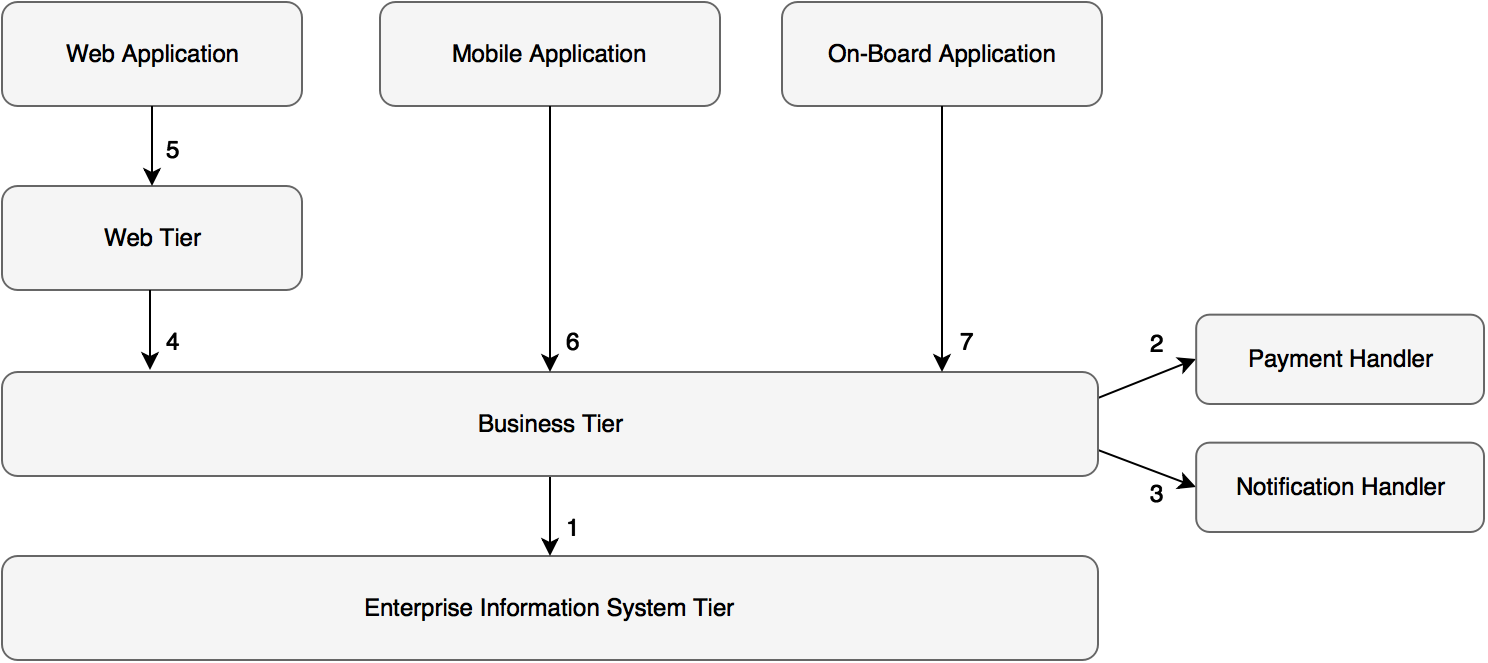
\includegraphics[width=1.0\textwidth]{/ITPD/subsystem_integration_sequence}\\
	  \vspace{0.2cm}
	  \caption{Integration sequence for the subsystems} 
	  \label{fig:subsystem_integration_sequence} 
	\end{figure}

	\begin{center}
		\vspace{0.6cm}
		\begin{tabular}{|l|l|l|}
			\hline
			\textbf{ID} & \textbf{Integration Test} & \textbf{Paragraphs} \bigstrut \\\hline
			\hline
			I11T1 & Business Tier \ensuremath{\rightarrow} Enterprise Information System Tier & \ref{I11}, \ref{TP3} \bigstrut \\\hline
			I12T1 & Business Tier \ensuremath{\rightarrow} Payment Handler & \ref{I12}, \ref{TP3} \bigstrut \\\hline
			I13T1 & Business Tier \ensuremath{\rightarrow} Notification Handler & \ref{I13}, \ref{TP3} \bigstrut \\\hline
			I14T1 & Web Tier \ensuremath{\rightarrow} Business Tier & \ref{I14}, \ref{TP3} \bigstrut \\\hline
			I15T1 & Web Application \ensuremath{\rightarrow} Web Tier & \ref{I15}, \ref{TP3} \bigstrut \\\hline
			I16T1 & Mobile Application \ensuremath{\rightarrow} Business Tier & \ref{I16}, \ref{TP3} \bigstrut \\\hline
			I17T1 & On-Board Application \ensuremath{\rightarrow} Business Tier & \ref{I17}, \ref{TP3} \bigstrut \\\hline
		\end{tabular}
	\end{center}

